%-----------------------------------------------------------------------------------------------------------------------------------------------%
%	The MIT License (MIT)
%
%	Copyright (c) 2015 Jan Küster
%
%	Permission is hereby granted, free of charge, to any person obtaining a copy
%	of this software and associated documentation files (the "Software"), to deal
%	in the Software without restriction, including without limitation the rights
%	to use, copy, modify, merge, publish, distribute, sublicense, and/or sell
%	copies of the Software, and to permit persons to whom the Software is
%	furnished to do so, subject to the following conditions:
%
%	THE SOFTWARE IS PROVIDED "AS IS", WITHOUT WARRANTY OF ANY KIND, EXPRESS OR
%	IMPLIED, INCLUDING BUT NOT LIMITED TO THE WARRANTIES OF MERCHANTABILITY,
%	FITNESS FOR A PARTICULAR PURPOSE AND NONINFRINGEMENT. IN NO EVENT SHALL THE
%	AUTHORS OR COPYRIGHT HOLDERS BE LIABLE FOR ANY CLAIM, DAMAGES OR OTHER
%	LIABILITY, WHETHER IN AN ACTION OF CONTRACT, TORT OR OTHERWISE, ARISING FROM,
%	OUT OF OR IN CONNECTION WITH THE SOFTWARE OR THE USE OR OTHER DEALINGS IN
%	THE SOFTWARE.
%
%
%-----------------------------------------------------------------------------------------------------------------------------------------------%


%============================================================================%
%
%	DOCUMENT DEFINITION
%
%============================================================================%

%we use article class because we want to fully customize the page and dont use a cv template
\documentclass[10pt,A4]{article}


%----------------------------------------------------------------------------------------
%	ENCODING
%----------------------------------------------------------------------------------------

%we use utf8 since we want to build from any machine
\usepackage[utf8]{inputenc}

%----------------------------------------------------------------------------------------
%	LOGIC
%----------------------------------------------------------------------------------------

% provides \isempty test
\usepackage{xifthen}

\usepackage{xstring,xifthen}

%----------------------------------------------------------------------------------------
%	FONT
%----------------------------------------------------------------------------------------

% some tex-live fonts - choose your own

%\usepackage[defaultsans]{droidsans}
%\usepackage[default]{comfortaa}
%\usepackage{cmbright}
%\usepackage[default]{raleway}
%\usepackage{fetamont}
%\usepackage[default]{gillius}
%\usepackage[light,math]{iwona}
\usepackage[thin]{roboto}

% set font default
\renewcommand*\familydefault{\sfdefault}
\usepackage[T1]{fontenc}

% more font size definitions
\usepackage{moresize}


%----------------------------------------------------------------------------------------
%	PAGE LAYOUT  DEFINITIONS
%----------------------------------------------------------------------------------------

%debug page outer frames
%\usepackage{showframe}


%define page styles using geometry
\usepackage[a4paper]{geometry}

% for example, change the margins to 2 inches all round
\geometry{top=1.75cm, bottom=-.6cm, left=1.5cm, right=1.5cm}

%use customized header
\usepackage{fancyhdr}
\pagestyle{fancy}

%less space between header and content
\setlength{\headheight}{-5pt}


%customize entries left, center and right
\lhead{}
\chead{ \small{Alex Ghiurău $\cdot$ 26/03/1992 $\cdot$ Software Engineer $\cdot$  Oradea, Romania $\cdot$  \textcolor{sectcol}{\textbf{alex.ghiurau@gmail.com}}  $\cdot$ +40 748 575 751}}
\rhead{}


%indentation is zero
\setlength{\parindent}{0mm}

%----------------------------------------------------------------------------------------
%	TABLE /ARRAY/LIST DEFINITIONS
%----------------------------------------------------------------------------------------

%for layouting tables
\usepackage{multicol}
\usepackage{multirow}

%extended aligning of tabular cells
\usepackage{array}

\newcolumntype{x}[1]{%
>{\raggedleft\hspace{0pt}}p{#1}}%

\usepackage{enumitem}


%----------------------------------------------------------------------------------------
%	GRAPHICS DEFINITIONS
%----------------------------------------------------------------------------------------

%for header image
\usepackage{graphicx}

%for floating figures
\usepackage{wrapfig}
\usepackage{float}
%\floatstyle{boxed}
%\restylefloat{figure}

%for drawing graphics
\usepackage{tikz}
\usetikzlibrary{shapes, backgrounds,mindmap, trees}


%----------------------------------------------------------------------------------------
%	Color DEFINITIONS
%----------------------------------------------------------------------------------------

\usepackage{color}

%accent color
\definecolor{bgcol}{RGB}{87, 117, 144}

%dark background color
\definecolor{sectcol}{RGB}{249, 132, 74}

%light background / accent color
\definecolor{softcol}{RGB}{243, 114, 44}


%============================================================================%
%
%
%	DEFINITIONS
%
%
%============================================================================%

%----------------------------------------------------------------------------------------
% 	HEADER
%----------------------------------------------------------------------------------------

% remove top header line
\renewcommand{\headrulewidth}{0pt}

%remove botttom header line
\renewcommand{\footrulewidth}{0pt}

%remove pagenum
\renewcommand{\thepage}{}

%remove section num
\renewcommand{\thesection}{}

%----------------------------------------------------------------------------------------
% 	ARROW GRAPHICS in Tikz
%----------------------------------------------------------------------------------------

% a six pointed arrow poiting to the left
\newcommand{\tzlarrow}{(0,0) -- (0.2,0) -- (0.3,0.2) -- (0.2,0.4) -- (0,0.4) -- (0.1,0.2) -- cycle;}

% include the left arrow into a tikz picture
% param1: fill color
%
\newcommand{\larrow}[1]
{\begin{tikzpicture}[scale=0.58]
	 \filldraw[fill=#1!100,draw=#1!100!black]  \tzlarrow
 \end{tikzpicture}
}

% a six pointed arrow poiting to the right
\newcommand{\tzrarrow}{ (0,0.2) -- (0.1,0) -- (0.3,0) -- (0.2,0.2) -- (0.3,0.4) -- (0.1,0.4) -- cycle;}

% include the right arrow into a tikz picture
% param1: fill color
%
\newcommand{\rarrow}
{
\begin{tikzpicture}[scale=0.7]
	\filldraw[fill=sectcol!100,draw=sectcol!100!black] \tzrarrow
 \end{tikzpicture}
}



%----------------------------------------------------------------------------------------
%	custom sections
%----------------------------------------------------------------------------------------

% create a coloured box with arrow and title as cv section headline
% param 1: section title
%
\newcommand{\cvsection}[1]
{
\colorbox{bgcol}{\makebox[1\linewidth][l]{
	\larrow{sectcol} \hspace{-8pt} \larrow{sectcol} \hspace{-8pt} \larrow{sectcol} \textcolor{white}{\textbf{#1}}\hspace{4pt}
}}\\
}

\newcommand\AddAdditional[1]{%
\StrLen{#1}[\MyStrLen]% we find the length of the string and store it in \MyStrLen
\ifthenelse{\equal{\MyStrLen}{1}}% we compare the length of the string with 1
{}{\larrow{bgcol} & #1 \\[2pt]}}

%create a coloured arrow with title as cv meta section section
% param 1: meta section title
%
\newcommand{\metasection}[2]{
	\begin{tabular*}{1\linewidth}{p{0.18\linewidth} p{0.76\linewidth}}
		\larrow{bgcol}\normalsize{\textbf{\textcolor{sectcol}{#1}}}&#2\\
	\end{tabular*}
}

%----------------------------------------------------------------------------------------
%	 CV EVENT
%----------------------------------------------------------------------------------------

% creates a stretched box as cv entry headline followed by two paragraphs about
% the work you did
% param 1:	event time i.e. 2014 or 2011-2014 etc.
% param 2:	event name (what did you do?)
% param 3:	institution (where did you work / study)
% param 4:	what was your position
% param 5:	some words about your contributions
%

\newcommand{\cvevent}[7] {
\begin{flushleft}
\textcolor{sectcol}{#1 - #3}\\
\textbf{#2}\\[-7pt]
\textcolor{softcol}{\hrule}
\vspace{\spread}
\begin{tabular*}{1\linewidth}{p{0.001\linewidth} p{0.9\linewidth}}
	\larrow{bgcol} & #4 \\[2pt]
	\larrow{bgcol} & #5 \\[\spread]
	\AddAdditional{#6}
\end{tabular*}
\end{flushleft}
%\textcolor{softcol}{\hrule}
}

% creates a stretched box as
\newcommand{\cveventmeta}[2] {
	\mbox{\mystrut \hspace{87pt}\textit{#1}}\\
	#2
}

%----------------------------------------------------------------------------------------
% CUSTOM STRUT FOR EMPTY BOXES
%----------------------------------------- -----------------------------------------------
\newcommand{\mystrut}{\rule[-.3\baselineskip]{0pt}{\baselineskip}}

%----------------------------------------------------------------------------------------
% CUSTOM LOREM IPSUM
%----------------------------------------------------------------------------------------
\newcommand{\lorem}
{Lorem ipsum dolor sit amet, consectetur adipiscing elit. Donec a diam lectus.}

%----------------------------------------------------------------------------------------
% SPREAD
%----------------------------------------------------------------------------------------
\newcommand{\spread}{7pt}

%============================================================================%
%
%
%
%	DOCUMENT CONTENT
%
%
%
%============================================================================%
\begin{document}


%use our custom fancy header definitions
\pagestyle{fancy}



\begin{minipage}[t]{0.485\textwidth}

\vspace{\spread}

%---------------------------------------------------------------------------------------
%	TITLE HEADLINE
%----------------------------------------------------------------------------------------

\hspace{-0.25\linewidth}\colorbox{bgcol}{\makebox[1.25\linewidth][c]{\HUGE{\textcolor{white}{\textsc{Alex}} } \textcolor{sectcol}{\rule[-1mm]{1mm}{0.9cm}} \HUGE{\textcolor{white}{\textsc{Ghiurău}} } }}

%----------------------------------------------------------------------------------------
%	HEADER IMAGE
%----------------------------------------------------------------------------------------
\hspace{-0.25\linewidth}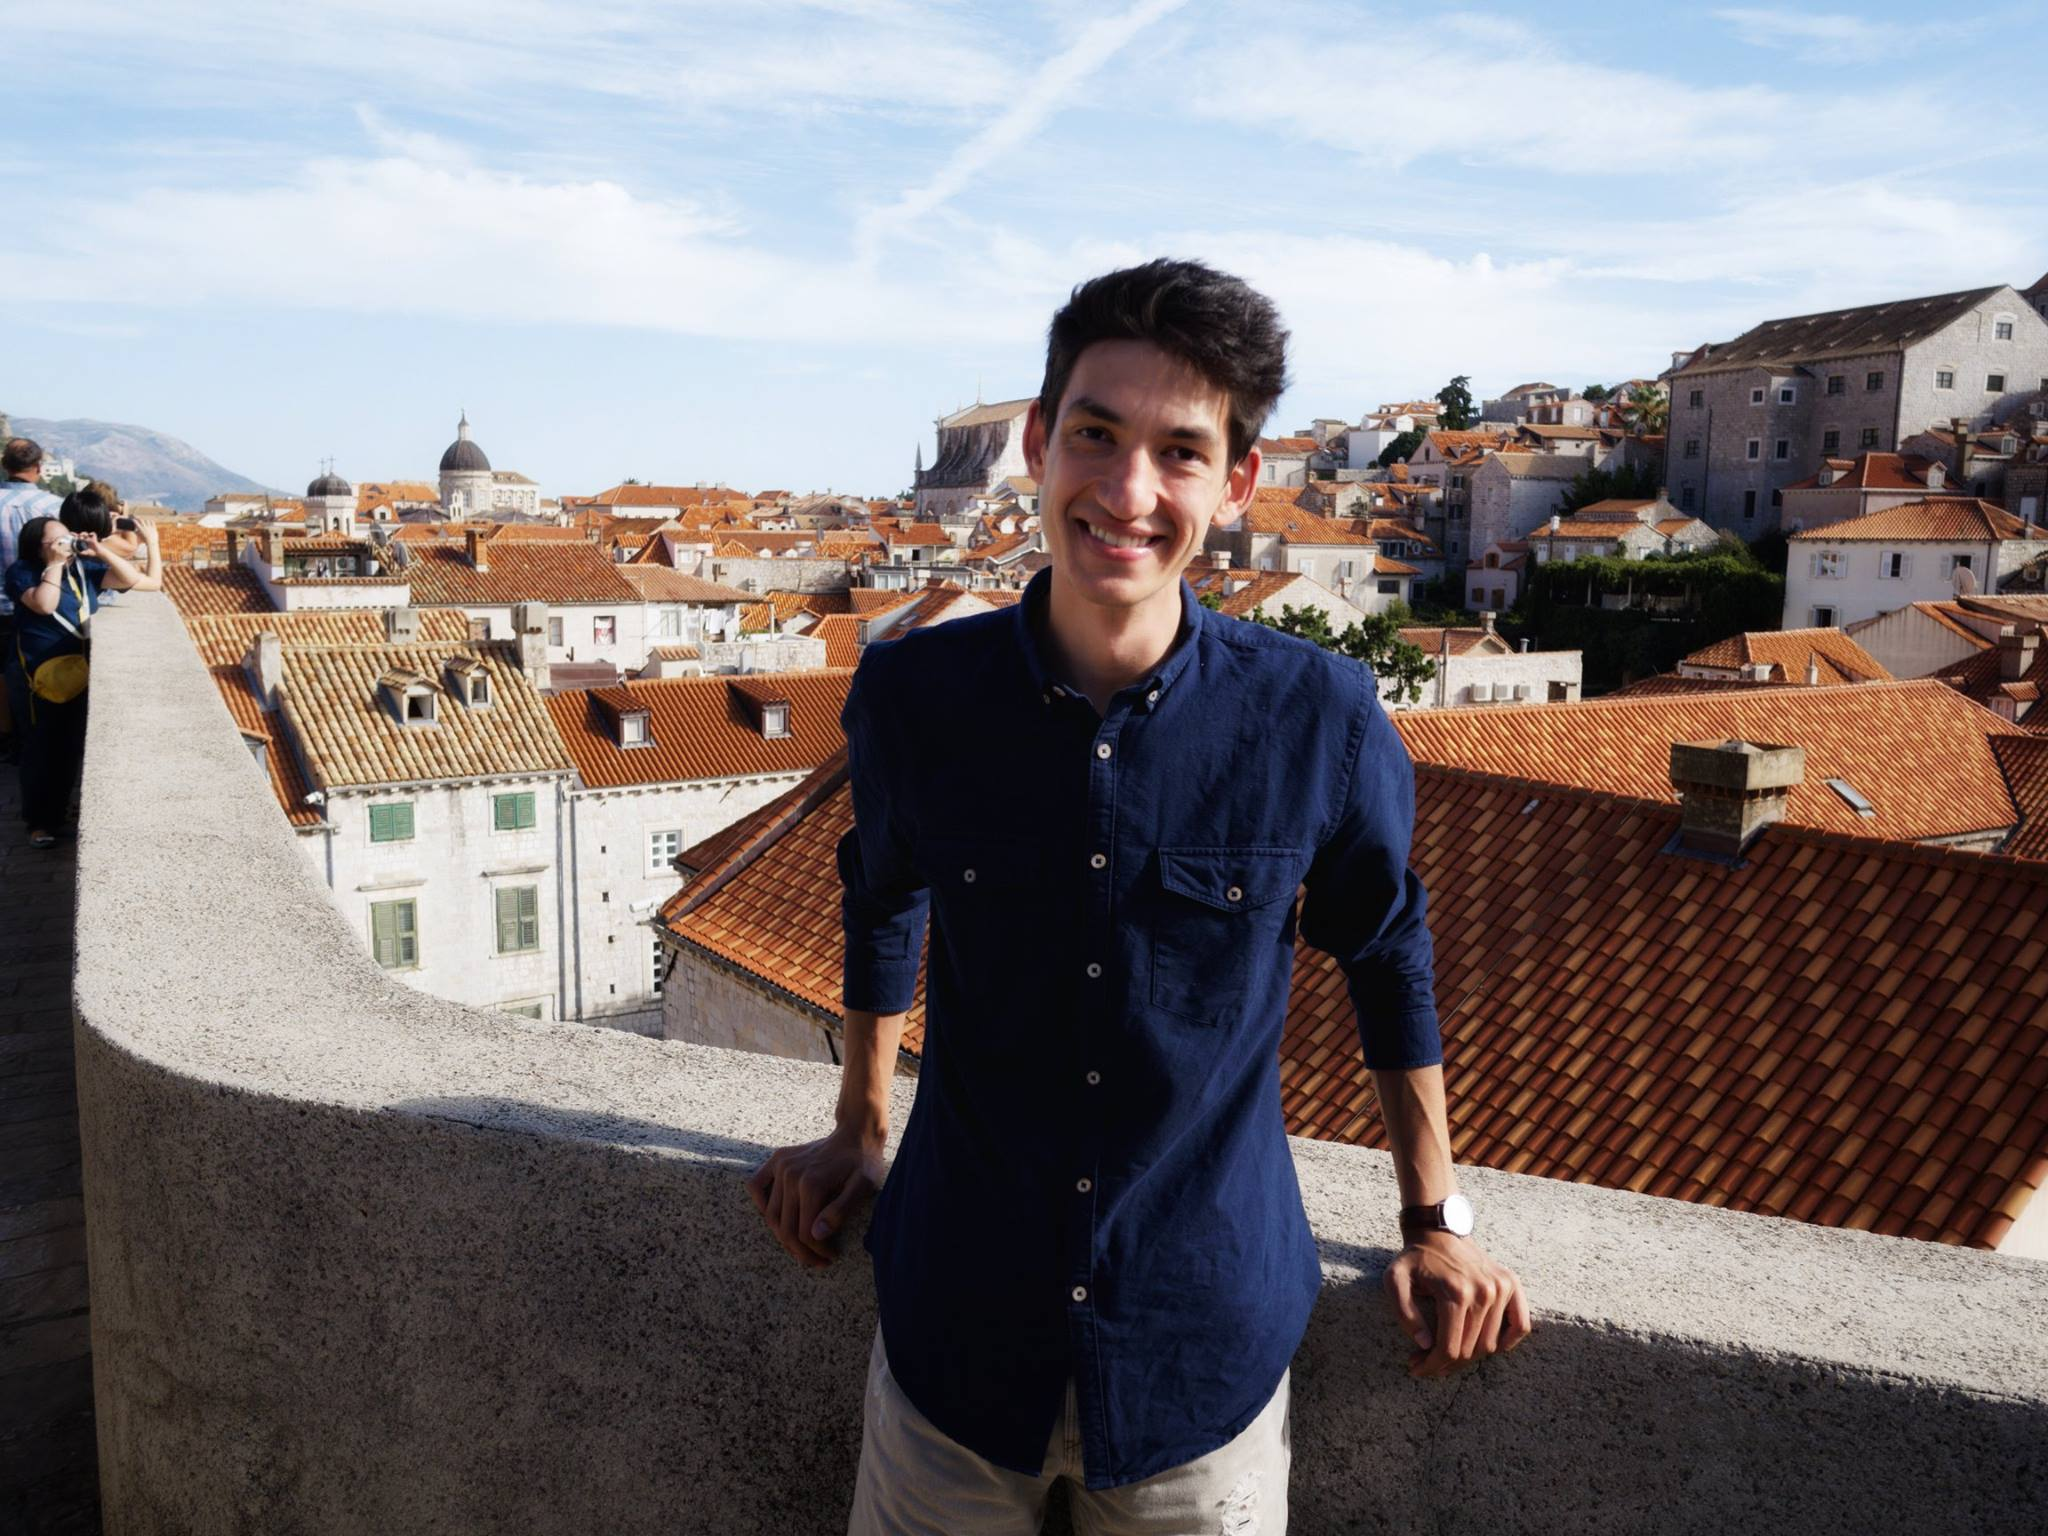
\includegraphics[width=1.2725\linewidth]{myfoto.jpg} %use full size

%---------------------------------------------------------------------------------------
%	QR CODE (optional)
%----------------------------------------------------------------------------------------
%\vspace{-100pt}
%\hspace{0.59\linewidth}
%
\includegraphics[width=88pt]{qrcode}
%\normalsize


\vspace{20pt}

\end{minipage}
\hfill
\begin{minipage}[t]{0.485\textwidth}
%---------------------------------------------------------------------------------------
%	SUMMARY (optional)
%----------------------------------------------------------------------------------------
\vspace{\spread}

\cvsection{Summary}\\
I am a networking \& telecommunications graduate (B.Sc.Eng) with project experience in the private sector. I worked at Digi Communications, also known as RCS \& RDS (romania communication systems - romania data systems), as a Tech Support for clients. \\
\\At Paymo I developed a mobile application that replicates the main functionalities of the webapp that is a Project Management SaaS, using React Native, GraphQL and other tools.\\
\\I recently developed a mobile radio app as a hobby, and have a couple of other ongoing projects. I also love hiking, taking photos of spectacular sceneries, cycling \& reading books during the weekends or whenever I get the chance.\\[-2pt]
\textcolor{softcol}{\hrule}

\end{minipage}

\begin{minipage}[t]{0.485\textwidth}

\vspace{\spread}

%---------------------------------------------------------------------------------------
%	META SECTION
%----------------------------------------------------------------------------------------
\metasection{Status:}{Fullstack JS Engineer, B.Sc.Eng - Networking \& Telecommunications}
\metasection{Fields:}{Project Management, Software Development, UX}
\end{minipage}
\hfill
\begin{minipage}[t]{0.485\textwidth}

\vspace{5pt}

\metasection{Tech:}{ Javascript - (React, Node, Extjs), ReactNative, Electron, GraphQL, MySQL, PHP, Git, PhpStorm, Sourcetree, AWS - (S3, CloudWatch)}
\metasection{Loves:}{Tech, Music, Cycling, Cars, Photography, Mountains, Books \& Tea}
\end{minipage}


\begin{minipage}[t]{0.485\textwidth}

\vspace{\spread}

%---------------------------------------------------------------------------------------
%	EDUCATION SECTION
%--------------------------------------------------------------------------------------

\cvsection{Education}

\cvevent{2015 / 07}{Graduated as B.S.E}{University of Oradea}{Bachelor Thesis: Software Application for monitoring an object using a Smartphone}{Developed a web application using rtsp/rtmp protocol that captures information from smartphone camera and streams it to a server}

%\textcolor{softcol}{\hrule}

%
\cvevent{2014 - 2014}{Informal School of IT}{Oradea Business Center}{Went through a web programming course}{Developed a basic site that required standard CRUD operations}

%\textcolor{softcol}{\hrule}

%
\cvevent{2011 - 2015}{B.Sc.Eng}{University of Oradea}{Studied networks \& telecommunications - networks infrastructures and got general knowledge in Matlab}{Programmed robots using Arduino, information visualization, professional essay writing}

%\textcolor{softcol}{\hrule}


\end{minipage}
\hfill
\begin{minipage}[t]{0.485\textwidth}

\vspace{\spread}

%---------------------------------------------------------------------------------------
%	EXPERIENCE
%----------------------------------------------------------------------------------------
\cvsection{Experience}

%
\cvevent{2017 - present}{Fullstack Javascript Engineer}{Paymo}
{Implement a Notifications Systems - a queued system that sends email notifications, in-app notifications, and mobile notifications (using Firebase) to concerned users using PHP Resque \& Redis}
{Develop a timer widget using Electron so that users can easily track time and add time entries from their desktop platforms}
{Develop a mobile app that resembles the web-app functionality using ReactNative, GraphQL \& other libraries}
{Create an onboarding progress tutorial for newly subscribed users using React}

%
\cvevent{2015 - 2016}{Junior Javascript Engineer}{Paymo}{Implement a File Uploader system that uploads in chunks on S3}{Restyle an old application using SCSS compiler \& give valuable UX advice}

%

\cvevent{2012 - 2015}{Tech Support / Customer Service Representative}{RCS-RDS}{Diagnose client problems and solve them via intern systems}{Add \& solve technical tickets}


\end{minipage}

%-------------------------------------------------------------------------------------------------
%	ARTIFICIAL FOOTER (fancy footer cannot exceed linewidth)
%--------------------------------------------------------------------------------------------------

\null
\vspace*{\fill}
\hspace{-0.25\linewidth}\colorbox{bgcol}{\makebox[1.5\linewidth][c]{\mystrut $\cdot$ \textcolor{white}{github.com/alexghi} $\cdot$ \textcolor{white}{https://www.linkedin.com/in/alex-ghiurau-048252b5/}}}




%============================================================================%
%
%
%
%	DOCUMENT END
%
%
%
%============================================================================%
\end{document}
